\begin{frame}
    \frametitle{Présentation générale}
  	\begin{block}{Historique}
  	\begin{itemize}
  		\item Japonais au XVIIIème siècle
  		\item Richard Dow (graphique) puis Nison (chandelier), Bollinger
	\end{itemize}
	
	\end{block}
	\pause
	\begin{block}{Définition}
		\begin{itemize}
			\item John Murphy : " L’analyse technique est l’étude de l’évolution d’un marché, principalement sur la base de graphiques, dans le but de prévoir les futures tendances ".
		\end{itemize}
	\end{block}
\end{frame}

\begin{frame}
    \frametitle{Tendances}
  	\begin{block}{Présentation}
  		Les lignes de tendances sont la loi de base de l’analyse technique :
  		\begin{itemize}
  			\item \textbf{La résistance} rejoint les points hauts de la courbe de valeur du cours.
  			\item \textbf{Le support} de même avec les points les plus bas
  		\end{itemize}
  		\center
  	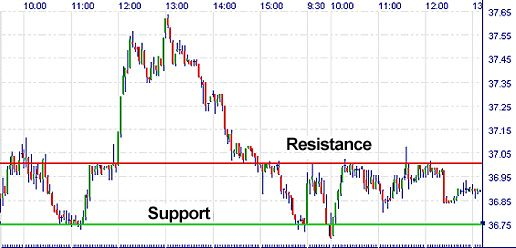
\includegraphics[scale=0.3]{images/supportresistance.jpg}

	\end{block}
\end{frame}

\begin{frame}
    \frametitle{Chandelier}
  

\end{frame}

\begin{frame}
    \frametitle{Chandelier}
  

\end{frame}

\begin{frame}
    \frametitle{Moyenne mobile}
  

\end{frame}

\begin{frame}
    \frametitle{Moyenne mobile}
  

\end{frame}

\begin{frame}
    \frametitle{Bollinger}
  

\end{frame}

\begin{frame}
    \frametitle{Bollinger}
  

\end{frame}

\begin{frame}
    \frametitle{Volume}
  

\end{frame}
